
%(BEGIN_QUESTION)
% Copyright 2011, Tony R. Kuphaldt, released under the Creative Commons Attribution License (v 1.0)
% This means you may do almost anything with this work of mine, so long as you give me proper credit

Les utvalgte deler av Siemens ``SIMATIC S7-200 Programmable Controller System Manual'' (dokument A5E00307987-04, august 2008) og svar på følgende spørsmål:

\vskip 10pt

Identifiser de ulike typene SIMATIC-\textit{timer}-instruksjoner, og forklar hvordan hver av dem fungerer.

\vskip 10pt

Identifiser en praktisk anvendelse for en timer-instruksjon programmert i en PLC.

\vskip 10pt

Hvor lenge kan én av disse timer-instruksjonene telle opp?  Basert på denne maksimumsverdien, hvor mange bit tror du brukes i registeret for å lagre timerinstruksjonens nåverdi?

\vskip 10pt

Hva menes med \textit{oppløsningen} til en timer-instruksjon?  Hvor mange forskjellige oppløsningsvalg tilbyr SIMATIC-instruksjonene?

\vskip 10pt

Kommenter hvordan verdien i en SIMATIC-timer oppdateres i et PLC-program når oppløsningen er 1 ms, når den er 10 ms, og når den er 100 ms.  Siemens S7-200 PLC håndterer disse ulikt!

\vskip 10pt

Skisser et enkelt stigeskjemaprogram for en Siemens S7-200 PLC der en bryter koblet til inngang {\tt I0.3} får en timer til å telle opp og deretter slår på en alarmlampeutgang {\tt Q0.9} etter 5 sekunder.

\vskip 20pt \vbox{\hrule \hbox{\strut \vrule{} {\bf Forslag til sokratisk diskusjon} \vrule} \hrule}

\begin{itemize}
\item{} Hvis du har tilgang til egen PLC for eksperimentering, anbefales det å skrive et enkelt \textit{demonstrasjonsprogram} som lar deg utforske oppførselen til disse PLC-instruksjonene.  Programmet trenger ikke gjøre noe nyttig, men bare demonstrere hva hver instruksjon gjør.  Les først relevant del av PLC-manualen eller instruksjonsreferansen for korrekt syntaks (f.eks. hvilke datatyper som brukes og hvilke adresser som er gyldige), og skriv deretter det enkleste programmet du kan for å demonstrere funksjonen isolert.  Last ned programmet til PLC-en, kjør det, og observer hvordan det fungerer ``live'' ved å se på fargemarkering i programmeringsverktøyet og/eller numeriske verdier som manipuleres av hver instruksjon.  Etter at du har ``leketøy'' med demonstrasjonsprogrammet og observert oppførselen, skriv kommentarer for hver rung som forklarer med egne ord hva hver instruksjon gjør.
\item{} Hvorfor tror du Siemens har designet timerinstruksjonene slik at nåverdien oppdateres forskjellig, avhengig av valgt oppløsning?  Hvorfor ikke la alle timerinstruksjoner oppdateres likt, uavhengig av oppløsning?
\end{itemize}

\underbar{file i00229}
%(END_QUESTION)





%(BEGIN_ANSWER)


%(END_ANSWER)





%(BEGIN_NOTES)

De tre SIMATIC-timerinstruksjonene er On-Delay Timer (TON), Retentive On-Delay Timer (TONR) og Off-Delay Timer (TOF).  Både TON og TONR teller tid når de er aktive; forskjellen er hva som skjer når inngangene deaktiveres: TON nullstilles umiddelbart, mens TONR beholder telleverdien.  TOF-timeren teller tid når inngangen deaktiveres.

SIMATIC-timerinstruksjoner kan nullstilles med en egen Reset-funksjon, som ser ut som en spoleinstruksjon med bokstaven ``R'' inni (tilsvarer Allen-Bradley sin ``RES''-spole).

\vskip 10pt

Disse timerne har en maksimal telleverdi på 32,767 (15-bit binært tall), med oppløsningene 1 ms, 10 ms og 100 ms.  For eksempel er telleverdi 5000 med 1 ms oppløsning lik 5000 millisekunder, altså 5 sekunder.  Samme telleverdi med 10 ms oppløsning er 50000 ms, altså 50 sekunder.

\vskip 10pt

Hvis oppløsningen til en timer er satt til 1 ms, oppdateres timertelleverdien gjennom hele programsveipet (dvs. flere ganger hvis sveiptiden overstiger 1 ms).  Dette betyr at timerens nåverdi kan endres på ulike steder i et stigeskjemaprogram.

Hvis oppløsningen er satt til 10 ms, oppdateres timerverdien ved starten av sveipsyklusen, og nåverdien forblir konstant gjennom resten av sveipet.

Hvis oppløsningen er satt til 100 ms, oppdateres timertelleverdien bare når timerinstruksjonen nås i programsveipet (side 198).

$$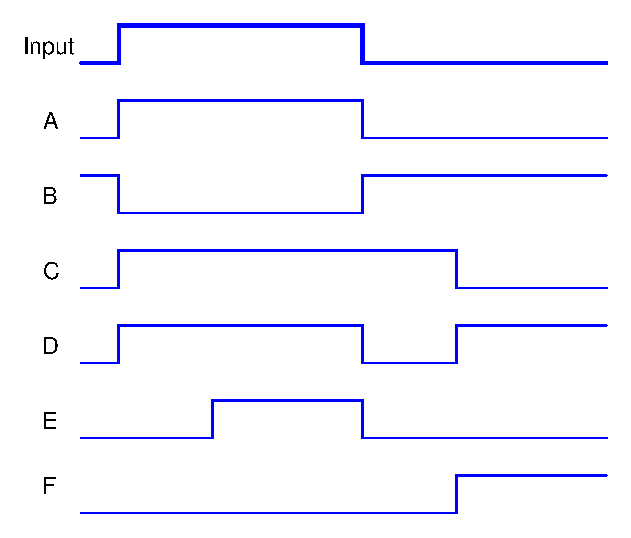
\includegraphics[width=15.5cm]{i00229x01.eps}$$

%INDEX% Reading assignment: Siemens S7-200 system manual (timer instructions)

%(END_NOTES)
